\section{Combinar}
\par{Este filtro permite reutilizar cálculos debido a dos factores. Uno de ellos es la forma que tiene cada píxel generado en la imagen resultante, que consiste en que si se tienen una imagen $A$ y una imagen $B$ de tamaño $m \times n$ entonces el píxel de la imagen generada ${I_{AB}}^{i, j}$ se calcula de la siguiente forma:}
\[ {I_{AB}}^{i,j} = \dfrac{\alpha * ( {I_{A}}^{i,j} - {I_{B}}^{i,j} )}{255.0} + {I_{B}}^{i,j} \]
\par{El otro factor es que nuestro filtro está optimizado para casos en los que la imagen $B$ es el reflejo vertical de la imagen $A$. Es decir que se da que ${I_{A}}^{i,j} = {I_{B}}^{i,n - j + 1}$ como se puede apreciar en la siguiente figura.}

\begin{figure}[h!]
\centering
\begin{minipage}{.5\textwidth}
\centering
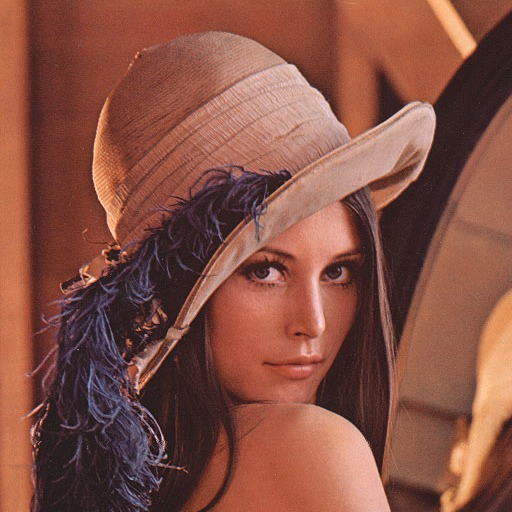
\includegraphics[width=5cm, height=5cm]{CombinarOriginal.jpg}
\label{}
\end{minipage}\hfill
\begin{minipage}{.5\textwidth}
\centering
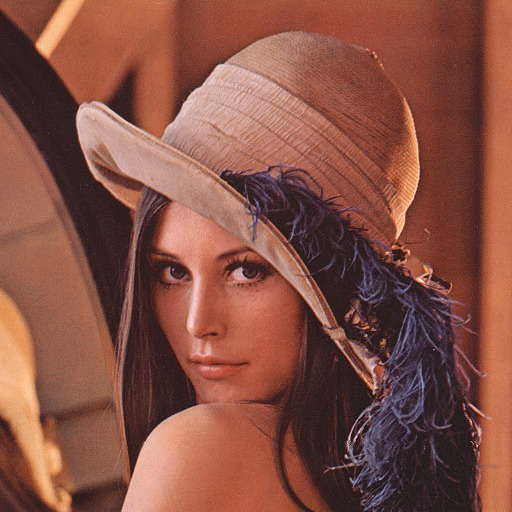
\includegraphics[width=5cm, height=5cm]{CombinarReflejo.jpg}
\label{}
\end{minipage}
\caption[center]{Se muestra la imagen $A$ del lado izquierdo con la imagen $B$, el reflejo vertical de A, en la parte derecha.}
\end{figure}

\par{Entonces se tiene que}
\begin{align}
{I_{AB}}^{i,j} &= \dfrac{\alpha * ( {I_{A}}^{i,j} - {I_{B}}^{i,j} )}{255.0} + {I_{B}}^{i,j} \textup{     por la fórmula del filtro} \nonumber \\
&= \dfrac{\alpha * ( {I_{A}}^{i,j} - {I_{A}}^{i,n - j + 1} )}{255.0} + {I_{A}}^{i,n - j + 1} \textup{    dado que} {I_{A}}^{i,j} = {I_{B}}^{i,n - j + 1}
\end{align}

y análogamente

\begin{align}
{I_{AB}}^{i,n - j + 1} &= \dfrac{\alpha * ( {I_{A}}^{i,n - j + 1} - {I_{B}}^{i,n - j +1} )}{255.0} + {I_{B}}^{i,n - j + 1}  \nonumber \\
&= \dfrac{\alpha * ( {I_{A}}^{i,n - j + 1} - {I_{A}}^{i,j} )}{255.0} + {I_{A}}^{i,j}
\end{align}

\par{Así, se obtiene}

\begin{align}
{I_{AB}}^{i,n - j + 1} &= -1 * \dfrac{\alpha * [-1 * ( {I_{A}}^{i,n - j + 1} - {I_{A}}^{i,j} )]}{255.0} - {I_{A}}^{i,n - j + 1} + {I_{A}}^{i,n - j + 1} + {I_{A}}^{i,j} \nonumber \\
&= -1 * \Big[ \dfrac{\alpha * ( {I_{A}}^{i,j} - {I_{A}}^{i,n - j + 1} )}{255.0} + {I_{A}}^{i,n - j + 1} \Big] + {I_{A}}^{i,n - j + 1} + {I_{A}}^{i,j} \nonumber \\
&= -1 * {I_{AB}}^{i,j} + {I_{A}}^{i,n - j + 1} + {I_{A}}^{i,j} \textup{usando la igualdad de (2)}
\end{align}

\par{Estos cálculos muestran que luego de hacer el procesamiento para generar un píxel de la parte izquierda de la imagen resultante se puede obtener el píxel que corresponde a la mitad derecha con pocos cálculos más. Más aún, si se denomina}
\[ P = \dfrac{\alpha * ( {I_{A}}^{i,j} - {I_{A}}^{i,n - j + 1} )}{255.0} \]
se consigue
\[ {I_{AB}}^{i,j} = P + {I_{A}}^{i,n - j + 1} \]
y
\[ {I_{AB}}^{i,n - j + 1} = -P + {I_{A}}^{i,j} \]
y son menos cálculos necesarios.

\subsection{Código C}
	
\subsection{Código ASM}
\par{}
	
	
\subsection{Experimentación}
\subsubsection{Idea}	

\subsubsection{Hipótesis}
	
	
\subsubsection{Resultados}
	
